\section{People}
\begin{wrapfigure}{R}{0.3\textwidth}
\centering
\vspace{-50pt}

\includegraphics[width=0.3\textwidth, keepaspectratio]{images/pact/people}
\caption{\label{fig:people}Hypothetical group of users.}
\vspace{-50pt}
\end{wrapfigure}
We will here make a short list of the different kinds of peoples in our target audience, and list some of the strengths and weaknesses and unique characteristics. 

\subsection{Independent Farmers}
\begin{wrapfigure}{R}{0.3\textwidth}
\centering
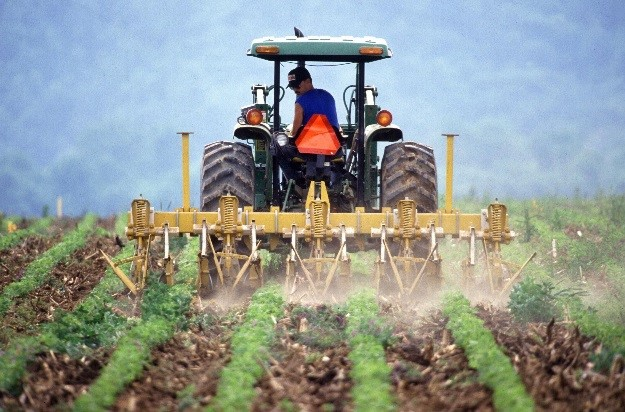
\includegraphics[width=0.3\textwidth, keepaspectratio]{images/pact/tractor}
\caption{\label{fig:independantfarmers}Picture of an independent farmer plowing a field.}
\vspace{-40pt}
\end{wrapfigure}
Independent Farmers need a way to keep track of recourse use of a particular field, and need to know the workload of the field as well. Farmers usually have a passing knowledge of new technology but is sometimes lacking in the application of those technologies.

\subsection{Organized farmers}
Organized farmers such as the company Arla have the same need as the independent farmer to keep track of either a single field of land or a whole slew of plots. Companies usually strife for profit maximization and minimal resource use. They are usually quick to apply new technology for that goal, and have organized rollout of those new technologies.

\subsection{Machinery contractors}
%\begin{wrapfigure}{R}{0.3\textwidth}
%\centering
%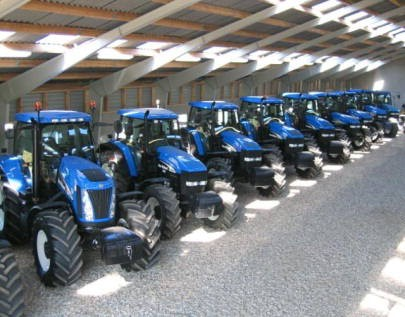
\includegraphics[width=0.3\textwidth, keepaspectratio]{images/pact/lotsoftractors}
%\caption{\label{fig:machinerycontractors}Picture of multiple tractors.}
%\end{wrapfigure}
Machinery contractors are companies that either rent out farm vehicles such as combines, or rent out the service wholesale where a famer rent the contractor to harvest a field for him. The contractors are interested in knowing how many resources a particular field need. This is so that they can help their customers’ needs and to find the right price. 
